 \chapter{ Descrição de uma rede neural tipo Perceptron}

  No campo da ciência da computação, temos um ramo de pesquisa que são as redes neuras artificias (RNAs), que são modelos computacionais que são influenciados no sistema nervoso central que tem habilidades de aprendizado. O exemplo de redes neurais são as redes perceptron, que são conectados às entradas por conjuntos de pesos.  Como melhor exemplificador pelas Figuras \ref{imagens:figura1} abaixo:  
  
  \begin{figure}[h!]
  	\label{imagens:figura1}
  	\centering
  	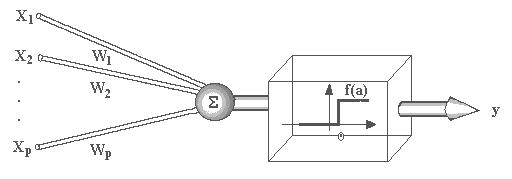
\includegraphics[width=0.55\linewidth]{imagens/Figura1.jpg}	
  	\caption{Ilustração rede perceptron de um neurônio.}
  \end{figure}
  
  Como podemos nota na Figura \ref{imagens:figura1} teremos um somatório do produtos entre as entradas, representada como $ x_{1}, x_{2} ... x_{p} $, e os pesos, é representada como $ w_{1}, w_{2} ... w_{p} $, %parei de edita aqui é calculada por cada nó de saída e, se o valor calculado ultrapassar um certo limiar (geralmente 0), o neurônio dispara e ajusta a saída para o valor 1; se o valor calculado é menor que o limiar, a saída é ajustada para o valor -1